% source: https://tex.stackexchange.com/questions/345420/how-to-draw-a-bloch-sphere

\documentclass{article}

\usepackage{tikz}
\usepackage{mathtools}
\usetikzlibrary{angles, quotes, arrows.meta}

\begin{document}
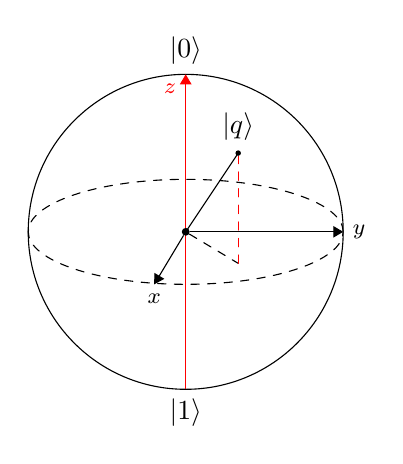
\begin{tikzpicture}[line cap=round, line join=round, >=Triangle]

    % Define radius
    \def\r{2}

    % Measurement axis
    \draw[red] (0, -\r) -- (0, \r);

    % Bloch vector
    \draw (0,0) node[circle, fill, inner sep=1] (orig) {}
    -- (\r/3,\r/2) node[circle, fill, inner sep=0.7, label=above:$|q\rangle$] (q) {};
    \draw[dashed] (orig) -- (\r/3, -\r/5);
    \draw[dashed, red] (\r/3, -\r/5) -- (q);

    % Sphere
    \draw (orig) circle (\r);
    \draw[dashed] (orig) ellipse (\r{} and \r/3);

    % Axes
    \draw[->] (orig) -- ++(-\r/5, -\r/3) node[below] (plus) {\footnotesize $x$};
    \draw[->] (orig) -- ++(\r, 0) node[right] (y) {\footnotesize $y$};
    \draw[->, red] (orig) -- ++(0, \r) node[anchor=north east] (z) {\footnotesize $z$};
    \draw (0, \r) node[above] (zero) {$|0\rangle$};
    \draw (0, -\r) node[below] (zero) {$|1\rangle$};

    % Angles
    % \pic [draw=gray, text=gray, ->, "$\phi$"] {angle = x1--orig--phi};
    % \pic [draw=gray, text=gray, <-, "$\theta$", angle eccentricity=1.4] {angle = a--orig--x3};

\end{tikzpicture}

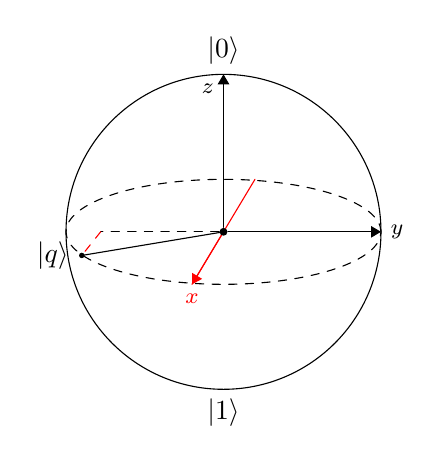
\begin{tikzpicture}[line cap=round, line join=round, >=Triangle]

    % Define radius
    \def\r{2}

    % Measurement axis
    \draw[red] (\r/5, \r/3) -- (-\r/5, -\r/3);

    % Bloch vector
    \draw (0,0) node[circle, fill, inner sep=1] (orig) {}
    -- (-0.9*\r,-0.15*\r) node[circle, fill, inner sep=0.7, label=left:$|q\rangle$] (q) {};
    \draw[dashed] (orig) -- (-0.78*\r, 0);
    \draw[dashed, red] (-0.78*\r, 0) -- (q);

    % Sphere
    \draw (orig) circle (\r);
    \draw[dashed] (orig) ellipse (\r{} and \r/3);

    % Axes
    \draw[->, red] (orig) -- (-\r/5, -\r/3) node[below] (plus) {\footnotesize $x$};
    \draw[->] (orig) -- ++(\r, 0) node[right] (y) {\footnotesize $y$};
    \draw[->] (orig) -- ++(0, \r) node[anchor=north east] (z) {\footnotesize $z$};
    \draw (0, \r) node[above] (zero) {$|0\rangle$};
    \draw (0, -\r) node[below] (zero) {$|1\rangle$};

    % Angles
    % \pic [draw=gray, text=gray, ->, "$\phi$"] {angle = x1--orig--phi};
    % \pic [draw=gray, text=gray, <-, "$\theta$", angle eccentricity=1.4] {angle = a--orig--x3};

\end{tikzpicture}
\end{document}